\documentclass{article}
\usepackage{graphicx} % Required for inserting images
\usepackage{setspace} % Double Space 
\usepackage{ragged2e} % justify text
\usepackage{enumitem} % enumeration within subsection
\usepackage{url} % inserting links and urls

\usepackage{pdflscape} % Horizontal page orientation
\usepackage{booktabs}  % For \toprule, \midrule and \bottomrule
\usepackage{float} 
\usepackage[spanish]{babel}

\usepackage[letterpaper, left=2cm, right=2cm, top=3cm, bottom=3cm]{geometry}

\setlength{\parskip}{1em} % we increase paragraph spacing

\title{Tesis}
\author{GUSTAVO ANDRES GONZALEZ PINEDA}
\date{February 2025}

\begin{document}

\begin{center}
\begin{doublespace}
    \thispagestyle{empty}  % no numbering for the cover
    \Large{UNIVERSIDAD DEL VALLE DE GUATEMALA}\\
    Facultad de Ingeniería \\    

    % Image placement
    \vspace{15mm} 
    
\includegraphics[width=0.2\textwidth]{images/Uvg_logo.jpg}

    \vspace{15mm} 
    {\Large Desarrollo de sistema de posicionamiento preciso en interiores mediante sensores UWB para recorridos virtuales con realidad aumentada en la Universidad del Valle de Guatemala.}

    \vspace{10mm} 
    {\Large Protocolo de Trabajo de graduación en modalidad de Trabajo Profesional presentado por Gustavo Andres González Pineda para optar al grado académico de Licenciado en Ingeniería en Ciencias de la Computación y Tecnologías de la Información.}

    {\Large Guatemala,  2025}
    
\end{doublespace}
\end{center}

\newpage % page left purposely on blank

\thispagestyle{empty} % Remove headers and footers (optional)
\mbox{} % Ensure the page is not optimized away
\newpage % Move to the next page


\begin{center}
\begin{doublespace}
    \thispagestyle{empty}  % no numbering for the cover
    \Large{UNIVERSIDAD DEL VALLE DE GUATEMALA}\\
    Facultad de Ingeniería \\    

    % Image placement
    \vspace{15mm} 
    
\includegraphics[width=0.2\textwidth]{images/Uvg_logo.jpg}

    \vspace{15mm} 
    {\Large Desarrollo de sistema de posicionamiento preciso en interiores mediante sensores UWB para recorridos virtuales con realidad aumentada en la Universidad del Valle de Guatemala.}

    \vspace{10mm} 
    {\Large Protocolo de Trabajo de graduación en modalidad de Trabajo Profesional presentado por Gustavo Andres González Pineda para optar al grado académico de Licenciado en Ingeniería en Ciencias de la Computación y Tecnologías de la Información.}

    {\Large Guatemala,  2025}
    
\end{doublespace}
\end{center}
% end of cover section

% begin table of contents
\tableofcontents
\newpage
% end table of contents

\setcounter{page}{1} % Start page numbering from page 1

\section{Abstract}
{\justify This project aims to develop a precise location system for an augmented reality application that guides users around the campus of the Universidad del Valle de Guatemala. The system is based on Estimote Beacons with Ultra-Wideband (UWB) technology and is designed to integrate with Unity through a native plugin that enables real-time communication between mobile devices and location sensors.

Unlike previous solutions that relied on QR codes or sensor fusion techniques subject to cumulative errors, this proposal employs Kalman filter-assisted trilateration to more reliably estimate the user's position in 2D coordinates. The system will be able to transmit this data to Unity, where it will be used to render augmented reality elements that guide the user around the campus.

The project is part of a larger ongoing initiative and focuses on the technical implementation of the positioning module, laying the groundwork for future cross-platform extensions. This technological solution significantly contributes to improving the on-campus wayfinding experience and represents an example of the practical use of emerging technologies in localization, signal filtering, and interactive mobile application development.}
\newpage

\section{Resumen}
{\justify
Este proyecto tiene como objetivo desarrollar un sistema de localización precisa para una aplicación de realidad aumentada que guía a los usuarios dentro del campus de la Universidad del Valle de Guatemala. El sistema se basa en sensores Estimote Beacons con tecnología Ultra-Wideband (UWB) y está diseñado para integrarse con Unity mediante un plugin nativo que permite la comunicación en tiempo real entre los dispositivos móviles y los sensores de localización.

A diferencia de soluciones anteriores que dependían de códigos QR o técnicas de sensor fusion sujetas a errores acumulativos, esta propuesta emplea trilateración asistida por filtros de Kalman para estimar con mayor estabilidad la posición del usuario en coordenadas 2D. El sistema será capaz de transmitir estos datos a Unity, donde se utilizan para renderizar elementos de realidad aumentada que guían al usuario por el campus.

El proyecto forma parte de una iniciativa mayor en curso y se enfoca en la implementación técnica del módulo de posicionamiento, sentando las bases para futuras extensiones multiplataforma. Esta solución tecnológica contribuye significativamente a mejorar la experiencia de orientación dentro del campus y representa un ejemplo del uso práctico de tecnologías emergentes en localización, filtrado de señales y desarrollo de aplicaciones móviles interactivas.
}
\newpage


\section{Introducción}
{\justify
La orientación dentro de un campus universitario puede representar un desafío para estudiantes nuevos, visitantes y personas con
 discapacidad. Con el avance de la tecnología, la realidad aumentada (AR) se ha convertido en una herramienta innovadora para mejorar
  la experiencia de navegación en espacios físicos. En este contexto, el presente proyecto busca desarrollar una aplicación de realidad
   aumentada para recorridos dentro de la Universidad del Valle de Guatemala (UVG), proporcionando una guía interactiva e inclusiva 
   que facilite el desplazamiento desde un punto A hasta un punto B dentro del campus.

Este proyecto se basa en el trabajo realizado en años anteriores, donde se implementó una versión preliminar de la navegación con AR,
 pero con limitaciones significativas. Una de las principales dificultades fue la dependencia de códigos QR para la ubicación, lo que
  restringía la precisión y fluidez del recorrido. Además, la implementación del algoritmo de pathfinding presentaba problemas en la 
  generación de rutas óptimas, afectando la experiencia del usuario.

Para mejorar estos aspectos, la universidad ha invertido en sensores Estimote Beacons con tecnología Ultra-Wideband (UWB), los cuales
 permitirán una localización más precisa dentro del campus. La labor de este trabajo se centrará en el mapeo del campus para 
 determinar la ubicación óptima de estos sensores, su configuración e integración con la aplicación y la optimización del algoritmo
  de pathfinding para generar rutas más accesibles y eficientes.

El objetivo es mejorar la precisión de la navegación y evitar rutas poco prácticas o inaccesibles para ciertos usuarios. Esto 
contribuirá a una experiencia más fluida y efectiva al desplazarse dentro del campus, garantizando que la aplicación proporcione 
indicaciones precisas y usables en diferentes escenarios.A través de este trabajo, se espera ofrecer una solución innovadora y 
funcional que aproveche las capacidades de la realidad aumentada y la localización UWB para facilitar la movilidad dentro de la UVG,
 mejorando la orientación y accesibilidad dentro del campus universitario.}
\newpage

\section{Objetivos}
\subsection{Objetivo general}
{\justify Desarrollar e implementar un plugin de localización en tiempo real mediante sensores Estimote con tecnología Ultra-Wideband (UWB), integrado a Unity, como parte de una aplicación de realidad aumentada que facilite los recorridos virtuales dentro del Centro de Innovación y Tecnología (CIT) del campus de la Universidad del Valle de Guatemala.}

\subsection{Objetivos específicos}
\begin{enumerate}[label=\thesubsection.\arabic*]
    \item Diseñar e implementar un algoritmo de trilateración
para estimar la posición bidimensional del usuario dentro del campus universitario,
mediante el procesamiento de las distancias medidas hacia múltiples sensores Estimote UWB distribuidos en el entorno.
    \item Integrar el SDK nativo de Estimote para iOS con Unity
para permitir la obtención y transferencia en tiempo real de datos de localización hacia la aplicación de realidad aumentada,
mediante el desarrollo de un plugin nativo en Swift que sirva de puente entre ambas plataformas.
    \item Aplicar técnicas de filtrado de señales
para mejorar la estabilidad del sistema de localización y reducir el efecto de ruido o jitter en las mediciones,
mediante la combinación de los datos obtenidos por trilateración y los registros del acelerómetro del dispositivo.
    \item Documentar el desarrollo del sistema de localización
para asegurar su mantenibilidad, facilitar su futura extensión a dispositivos Android y permitir su continuidad,
mediante la elaboración de documentación técnica clara sobre la arquitectura del plugin, las decisiones de diseño y los procesos de integración.
    \item Evaluar cualitativamente la precisión y suavidad del sistema de localización
para validar su funcionamiento en condiciones reales y su aporte a la experiencia de usuario dentro de la aplicación,
mediante la observación directa del comportamiento del sistema y el análisis de las distribuciones de datos de posición obtenidas durante pruebas manuales.       
\end{enumerate}

\newpage

\section{Justificación}
{\justify
Actualmente, el proceso de orientación para estudiantes nuevos, visitantes y padres de familia dentro del campus universitario de la Universidad del Valle de Guatemala presenta diversas limitaciones. Tradicionalmente, el recorrido por las instalaciones es guiado por estudiantes o personal universitario, pero este se realiza una única vez —si es que se llega a realizar— lo cual suele ser insuficiente para que los usuarios recuerden rutas, espacios o servicios disponibles. Como consecuencia, durante los primeros semestres, muchos estudiantes enfrentan dificultades para ubicarse, llegando a perderse o desaprovechar recursos valiosos del campus.

Además de la desorientación inicial, existen barreras de accesibilidad que afectan a personas con movilidad reducida o con discapacidades visuales, quienes podrían beneficiarse significativamente de un sistema que les permita planificar sus trayectos de forma precisa y adaptada a sus necesidades. Una solución tecnológica puede contribuir a solventar ambos problemas, mejorando tanto la orientación como la inclusión dentro del entorno universitario.

En este contexto, el desarrollo de una aplicación de realidad aumentada con capacidades de localización y navegación precisa representa una oportunidad para aplicar conocimientos técnicos adquiridos a lo largo de la carrera de Ingeniería en Ciencias de la Computación y Tecnologías de la Información. Este proyecto integra áreas clave como programación orientada a objetos, interacción humano-computadora, gráficos por computadora, desarrollo móvil y algoritmos de búsqueda de caminos (pathfinding). Asimismo, se utilizarán sensores Estimote Beacons con tecnología Ultra-Wideband (UWB), cuya precisión y facilidad de conexión brindan una ventaja considerable en comparación con tecnologías previamente utilizadas, como los códigos QR.

Este trabajo, al ser parte de un megaproyecto en curso, busca fortalecer y mejorar la versión previa de la aplicación desarrollada por generaciones anteriores, proponiendo avances significativos en la precisión de la localización y en la experiencia del usuario. La solución no solo resolverá problemas existentes, sino que también funcionará como base tecnológica para futuras generaciones de estudiantes que podrán continuar desarrollando y afinando la herramienta.

Finalmente, este proyecto aporta a la universidad al fortalecer su imagen como institución innovadora, capaz de generar soluciones tecnológicas útiles y vanguardistas dentro de su propio entorno. Comunica el potencial de sus estudiantes para abordar problemas reales mediante el uso creativo y riguroso del conocimiento adquirido, posicionando a la UVG como una universidad comprometida con la tecnología, la accesibilidad y la experiencia estudiantil.}

\newpage
\section{Marco Teórico}
\subsection{Localización en interiores}
{\justify La localización en interiores, también conocida como Indoor Positioning, es un área de estudio dentro de la computación ubicua que busca determinar la posición de personas u objetos dentro de espacios cerrados, donde las señales satelitales como el GPS pierden cobertura o presentan alta inexactitud. A diferencia de los sistemas de localización en exteriores, la implementación de soluciones en interiores implica múltiples retos técnicos, como la interferencia de estructuras físicas (paredes, techos, mobiliario), el comportamiento impredecible de las señales de radiofrecuencia por efectos como la reflexión, refracción y difracción, así como la variabilidad en el entorno.

Para suplir estas limitaciones, se han explorado diferentes tecnologías de localización alternativas, entre ellas Wi-Fi, Bluetooth Low Energy (BLE), RFID, visión por computadora y Ultra-Wideband (UWB). Cada tecnología ofrece un compromiso distinto entre precisión, consumo energético, costo y complejidad de implementación. En entornos que requieren alta precisión —como hospitales, bodegas o, en este caso, instalaciones universitarias complejas—, el UWB se destaca por ofrecer ventajas clave frente a sus competidores, sobre todo en términos de exactitud, latencia y robustez frente al ruido ambiental.}


\subsection{Tecnología Ultra-Wideband (UWB)}
{\justify La tecnología Ultra-Wideband (UWB) se basa en el uso de pulsos de muy corta duración que se propagan en un espectro extremadamente amplio (mayor a 500 MHz). Esta característica permite transmitir datos con alta precisión temporal, lo que a su vez facilita la medición del tiempo exacto que tarda una señal en desplazarse entre dos dispositivos. A través de estos tiempos de vuelo (Time of Flight, ToF), un receptor puede estimar con mucha precisión la distancia a un emisor, sin depender de la intensidad de la señal (RSSI), como ocurre en tecnologías menos precisas como BLE o Wi-Fi.

En aplicaciones de localización, los dispositivos UWB se colocan en el entorno como anclas o beacons, que transmiten pulsos periódicamente. Un dispositivo móvil equipado con un receptor UWB puede calcular su distancia a múltiples beacons y usar dicha información para estimar su posición. Esta técnica, que combina alta precisión (en el orden de decímetros o incluso centímetros) con baja latencia, es ideal para aplicaciones donde se requiere posicionamiento en tiempo real con gran fidelidad espacial, como la navegación asistida con realidad aumentada. En este proyecto se utilizan sensores Estimote UWB Beacons, diseñados específicamente para tareas de localización en interiores, con soporte en plataformas móviles como iOS.}


\subsection{Trilateración}
{\justify La trilateración es un método geométrico fundamental en sistemas de localización que permite calcular la posición de un punto desconocido en el espacio utilizando las distancias conocidas a tres o más puntos de referencia cuyas ubicaciones son fijas. En el caso de localización en dos dimensiones, si se conocen las coordenadas de tres sensores (beacons) y las distancias del dispositivo móvil a cada uno de ellos, es posible determinar su posición mediante la intersección de los tres círculos generados por esas distancias. En la práctica, debido a errores de medición, estas circunferencias rara vez se intersectan en un solo punto, por lo que se recurre a métodos de optimización y regresión para encontrar el punto más probable.

Cuando se disponen más de tres sensores, se puede aplicar trilateración redundante, técnica que permite mejorar la estabilidad de la estimación al reducir el impacto de errores individuales en las mediciones. La trilateración es la base matemática de muchos sistemas de localización, incluidos GPS, y en este proyecto, se adapta al contexto del campus universitario, utilizando coordenadas cartesianas en un plano 2D para determinar la ubicación del usuario en tiempo real.}

\subsection{ Filtro de Kalman}
{\justify El filtro de Kalman es un algoritmo recursivo de estimación desarrollado por Rudolf E. Kálmán en la década de 1960, utilizado para predecir el estado de un sistema dinámico y corregir esa predicción a partir de mediciones ruidosas. Su aplicación ha sido clave en campos como la navegación inercial, la robótica, el seguimiento de objetos y los sistemas de control, debido a su capacidad para integrar múltiples fuentes de información en presencia de incertidumbre.

En el contexto de este proyecto, el filtro de Kalman se emplea para suavizar la trayectoria estimada del usuario dentro del campus, combinando las posiciones calculadas mediante trilateración con los datos del acelerómetro del dispositivo móvil. Esta fusión sensorial permite reducir el jitter, es decir, las pequeñas oscilaciones aleatorias en la posición del usuario, y mejorar la estabilidad de la trayectoria percibida. Aunque el sistema no busca una precisión milimétrica absoluta, el objetivo es proporcionar una experiencia de navegación fluida, donde la posición calculada varíe de forma coherente con el movimiento del usuario.}

\subsection{Acelerómetro}
{\justify El acelerómetro es un sensor electrónico capaz de medir la aceleración de un cuerpo en los tres ejes del espacio (x, y, z), tanto por efecto del movimiento como por la fuerza gravitacional. En los dispositivos móviles modernos, los acelerómetros permiten funciones como la detección de orientación, el conteo de pasos, y la navegación sin GPS (dead reckoning).

En este proyecto, el acelerómetro se utiliza como complemento a la trilateración UWB para mejorar la estimación de la posición del usuario. Aunque los acelerómetros presentan el inconveniente de la deriva acumulativa (pequeños errores que se amplifican con el tiempo cuando se integra la aceleración), su uso combinado con los datos de distancia de los sensores UWB, mediante el filtro de Kalman, permite detectar transiciones suaves en el movimiento del usuario, anticipar su dirección y estabilizar la trayectoria. De esta manera, el sistema puede ofrecer una experiencia más coherente y natural en la navegación con realidad aumentada.}

\subsection{Unity y Realidad Aumentada}
{\justify Unity es un motor de desarrollo multiplataforma ampliamente utilizado en la industria de los videojuegos, simulaciones y aplicaciones interactivas. Su compatibilidad con dispositivos móviles y su integración con librerías de realidad aumentada como ARKit (iOS) y ARCore (Android), lo convierten en una herramienta poderosa para el desarrollo de experiencias inmersivas en tiempo real.

En este proyecto, Unity se emplea como el entorno de ejecución principal para la aplicación de recorridos virtuales con realidad aumentada. A través de la cámara del dispositivo móvil, el usuario puede observar su entorno mientras el sistema le sobreimpone elementos gráficos —como flechas tridimensionales— que le indican hacia dónde debe avanzar para completar un recorrido. La interacción entre estos elementos visuales y el sistema de localización precisa permite convertir el espacio físico del campus en una experiencia guiada interactiva, intuitiva y accesible.}

\subsection{Plugins Nativos para Unity (iOS)}
{\justify Debido a que Unity no ofrece acceso directo a todas las funcionalidades del sistema operativo, como sensores especializados o bibliotecas nativas, es común extender su funcionalidad mediante plugins nativos. Un plugin nativo permite conectar el código de Unity con código escrito en lenguajes como Swift (para iOS) o Kotlin (para Android), habilitando el uso de SDKs que solo están disponibles de forma nativa.

En el caso de este proyecto, se desarrolla un plugin en Swift que se encarga de establecer la comunicación con los sensores Estimote UWB, procesar las mediciones de distancia, acceder a los datos del acelerómetro mediante el framework CoreMotion, realizar los cálculos de trilateración y aplicar el filtro de Kalman. Este plugin se comunica con Unity a través de una interfaz de funciones expuestas, enviando las coordenadas calculadas para ser usadas por el motor gráfico en la navegación. Esta arquitectura modular garantiza que el sistema pueda mantenerse y extenderse fácilmente, incluyendo la posibilidad futura de implementar un plugin análogo para Android.}
\newpage

\section{Metodología}
\subsection{Introducción}


Para alcanzar los objetivos planteados en este proyecto, se ha diseñado una metodología de carácter \textbf{experimental}, centrada en la integración de sensores UWB, el desarrollo de plugins nativos para iOS y su comunicación con el motor gráfico Unity. El enfoque se basa en el diseño, implementación, prueba y ajuste de algoritmos y módulos de software dentro de un entorno controlado y real, específicamente el edificio del Centro de Innovación y Tecnología de la Universidad del Valle de Guatemala.

\subsection{Tipo de investigación}

La investigación es de tipo \textbf{experimental aplicada}, ya que se basa en la validación empírica de una solución tecnológica diseñada para resolver un problema específico del entorno universitario. A través de pruebas funcionales, análisis de datos y evaluación cualitativa, se busca comprobar la viabilidad y efectividad de un sistema de localización en tiempo real, integrable con una aplicación de realidad aumentada.

\subsection{Metodología estructurada por objetivos}

\subsubsection{Objetivo 1: Diseñar e implementar un algoritmo de trilateración para estimar la posición 2D del usuario}


\begin{itemize}
    \item \textbf{Fase 1: Diseño del algoritmo} \\
    Se definirá un modelo matemático basado en trilateración 2D utilizando coordenadas cartesianas. El algoritmo tomará como entrada las distancias a múltiples sensores UWB y devolverá una estimación de posición en el plano.

    \item \textbf{Fase 2: Desarrollo del algoritmo} \\
    El algoritmo será implementado en Swift como parte del plugin nativo para iOS. Se probará inicialmente en entornos controlados utilizando distancias simuladas y luego con datos reales de los sensores Estimote.

    \item \textbf{Fase 3: Validación funcional} \\
    Se realizarán pruebas en campo para verificar la estabilidad del algoritmo, observando la coherencia espacial de las posiciones calculadas frente al movimiento del usuario.
\end{itemize}

\subsubsection{Herramientas y conocimientos aplicados:} Para el desarrollo de este objetivo se aplican {\justify conocimientos de geometría analítica para modelar matemáticamente la trilateración en dos dimensiones, utilizando coordenadas cartesianas. Asimismo, se emplea programación orientada a objetos en el lenguaje Swift para implementar el algoritmo dentro de un entorno nativo para iOS. Se recurre también a principios básicos de teoría de localización y análisis espacial para interpretar las relaciones entre sensores y usuario, y garantizar que los cálculos de posición tengan coherencia estructural en un espacio real.}

\subsubsection{Objetivo 2: Integrar el SDK nativo de Estimote con Unity mediante un plugin de comunicación en tiempo real}

\begin{itemize}
    \item \textbf{Fase 1: Conexión con sensores UWB} \\
    Se desarrollará un módulo nativo en Swift capaz de escanear, conectar y recibir datos de los sensores Estimote UWB, utilizando el SDK oficial proporcionado por el fabricante.

    \item \textbf{Fase 2: Desarrollo del plugin para Unity} \\
    Se diseñará un plugin nativo que actúe como puente entre el código Swift y el entorno Unity, permitiendo transmitir datos de posicionamiento en tiempo real.

    \item \textbf{Fase 3: Validación de la comunicación} \\
    Se probará la integración verificando la correcta recepción y actualización de coordenadas dentro de Unity, así como el rendimiento del sistema en condiciones reales de uso.
\end{itemize}

\subsubsection{Herramientas y conocimientos aplicados:} 
{\justify Este objetivo requiere la aplicación de conocimientos en desarrollo móvil nativo, específicamente para iOS, a través del uso de Swift y del SDK oficial de Estimote para sensores UWB. Además, se requiere dominio de la integración de plugins nativos en Unity, lo cual implica comprender los mecanismos de interoperabilidad entre plataformas, la comunicación entre código nativo y el motor gráfico, y el paso eficiente de datos en tiempo real. También se aplican conceptos de diseño modular y arquitectura de software para estructurar el plugin de forma mantenible.}

\subsubsection{Objetivo 3: Aplicar filtrado con técnicas como el filtro de Kalman para reducir el jitter}

\begin{itemize}
    \item \textbf{Fase 1: Recolección de datos crudos} \\
    Se recopilarán datos en tiempo real de la trilateración y del acelerómetro del dispositivo móvil mediante CoreMotion.

    \item \textbf{Fase 2: Implementación del filtro de Kalman} \\
    Se desarrollará un módulo en Swift que aplique el filtro de Kalman a las posiciones estimadas, utilizando como entradas tanto las mediciones UWB como la aceleración registrada.

    \item \textbf{Fase 3: Análisis de estabilidad} \\
    Se evaluará la efectividad del filtrado mediante visualización de trayectorias y análisis del ruido residual en las posiciones. Se priorizará la precisión (consistencia) sobre la exactitud absoluta.
\end{itemize}

\subsubsection{Herramientas y conocimientos aplicados:} 
{\justify En este punto del proyecto se aplican fundamentos de estadística aplicada y procesamiento de señales para implementar técnicas de filtrado, con énfasis en el filtro de Kalman. También se integran conceptos relacionados con sensores inerciales como el acelerómetro y giroscopio, usando librerías como CoreMotion en iOS para complementar los datos de posición. Finalmente, se requiere la capacidad de programar estructuras de filtrado en tiempo real y analizar la relación entre precisión, estabilidad y ruido de la señal.}

\subsubsection{Objetivo 4: Documentar el desarrollo del plugin y su integración}

\begin{itemize}
    \item \textbf{Fase 1: Estructuración del código y módulos} \\
    Se organizará el código del plugin de manera modular y reutilizable, con comentarios explicativos y convenciones de nomenclatura claras.

    \item \textbf{Fase 2: Elaboración de documentación técnica} \\
    Se redactará documentación detallada que describa la arquitectura del sistema, el funcionamiento interno del plugin, los flujos de datos y los pasos para su integración y reutilización.

    \item \textbf{Fase 3: Publicación y entrega} \\
    Toda la documentación será entregada junto al proyecto final y se dispondrá para futuras generaciones con el fin de facilitar la continuidad del megaproyecto.
\end{itemize}

\subsubsection{Herramientas y conocimientos aplicados:} 
{\justify Para este objetivo se aplican buenas prácticas de desarrollo de software, como la escritura de código modular, comentado y con convenciones claras de nomenclatura. También se emplean técnicas de documentación técnica para describir el funcionamiento de cada módulo, la estructura del sistema, los flujos de datos y los pasos necesarios para su mantenimiento o extensión. Todo esto se enmarca dentro de un enfoque de diseño sostenible, que busca facilitar la transferencia del conocimiento a futuros desarrolladores del megaproyecto.}

\subsubsection{Objetivo 5: Evaluar cualitativamente la precisión y suavidad del sistema de localización}

\begin{itemize}
    \item \textbf{Fase 1: Pruebas de campo} \\
    Se ejecutarán pruebas en zonas específicas del edificio para observar el comportamiento del sistema en movimiento y en reposo.

    \item \textbf{Fase 2: Recolección y análisis de datos} \\
    Se analizarán trayectorias, jitter, y ruido en las posiciones generadas. Se observará la estabilidad visual del sistema para el usuario final.

    \item \textbf{Fase 3: Ajustes iterativos} \\
    En caso de detectar irregularidades, se realizarán ajustes al algoritmo de trilateración o al filtro de Kalman hasta alcanzar una experiencia fluida.
\end{itemize}

\subsubsection{Herramientas y conocimientos aplicados:} 
{\justify En esta etapa se aplican conocimientos de análisis de datos para interpretar trayectorias, identificar patrones de jitter y evaluar la continuidad del movimiento estimado por el sistema. Se utilizan herramientas de visualización para representar el comportamiento del sistema bajo diferentes condiciones de uso. También se recurre a métodos de prueba empírica y ajuste de parámetros para afinar el sistema con base en los resultados observados, priorizando una experiencia fluida por encima de una exactitud matemática absoluta.}

\subsection{Recolección de datos}

Durante el desarrollo y validación del sistema se recopilarán los siguientes tipos de datos:

\begin{itemize}
    \item Distancias entre el dispositivo móvil y sensores UWB.
    \item Coordenadas calculadas por el sistema de trilateración.
    \item Aceleración y orientación medidas por el acelerómetro y giroscopio del dispositivo.
    \item Registros de estabilidad (jitter) y continuidad de la trayectoria estimada.
\end{itemize}

Todas las pruebas se llevarán a cabo dentro del campus universitario en condiciones controladas, utilizando dispositivos iOS compatibles con UWB.

\subsection{Análisis de datos}

El análisis de datos se enfocará en:

\begin{itemize}
    \item Cuantificar la estabilidad de las posiciones calculadas en reposo y en movimiento.
    \item Visualizar trayectorias para detectar ruido o errores de salto.
    \item Comparar el comportamiento del sistema con y sin filtrado aplicado.
\end{itemize}

Se utilizarán herramientas de análisis visual y gráficos generados mediante scripts personalizados en Swift o Python, según se requiera.

\subsection{Consideraciones éticas}

Este proyecto no involucra usuarios reales en esta etapa, ni recopila información sensible. Sin embargo, se contemplan las siguientes buenas prácticas para futuras fases o generaciones:

\begin{itemize}
    \item Solicitar consentimiento informado si se realizan pruebas con participantes.
    \item Garantizar el anonimato de los datos de localización recolectados.
    \item Usar la información únicamente con fines académicos y de mejora del sistema.
\end{itemize}

Actualmente, todos los datos son técnicos y recopilados internamente por los desarrolladores en contextos controlados.
\newpage

\section{Índice Preliminar}


\begin{itemize}
  \item 1. Lista de cuadros y figuras
  \item 2. Resumen
  \item 3. Abstract
  \item 4. Introducción
  \item 5. Antecedentes del megaproyecto
  \item 6. Justificación
  \item 7. Objetivos
  \begin{itemize}
    \item 7.1 Objetivo general
    \item 7.2 Objetivos específicos
  \end{itemize}
  \item 8. Marco Teórico
  \begin{itemize}
    \item 8.1 Tecnologías de localización en interiores
    \begin{itemize}
      \item 8.1.1 UWB vs BLE vs GPS
      \item 8.1.2 Sensores Estimote y su integración en dispositivos móviles
    \end{itemize}
    \item 8.2 Algoritmos de localización
    \begin{itemize}
      \item 8.2.1 Trilateración en 2D
      \item 8.2.2 Filtros de Kalman aplicados a la navegación
    \end{itemize}
    \item 8.3 Realidad aumentada con Unity
    \begin{itemize}
      \item 8.3.1 AR Foundation
      \item 8.3.2 Desarrollo de plugins nativos para Unity (iOS/Android)
      \item 8.3.3 Comunicación entre capas nativas y Unity
    \end{itemize}
  \end{itemize}
  \item 9. Metodología
  \begin{itemize}
    \item 9.1 Tipo de investigación
    \item 9.2 Metodología estructurada por objetivos
    \begin{itemize}
      \item 9.2.1 Objetivo específico 1: Algoritmo de trilateración
      \item 9.2.2 Objetivo específico 2: Integración del SDK nativo
      \item 9.2.3 Objetivo específico 3: Filtro de Kalman
      \item 9.2.4 Objetivo específico 4: Documentación técnica
      \item 9.2.5 Objetivo específico 5: Evaluación cualitativa del sistema
    \end{itemize}
    \item 9.3 Recolección de datos
    \item 9.4 Análisis de datos
    \item 9.5 Consideraciones éticas
  \end{itemize}  
  \item 10. Resultados
  \item 11. Discusión
  \item 12. Conclusiones
  \item 13. Recomendaciones
  \item 14. Bibliografía
  \item 15. Anexos
  \item 16. Glosario
\end{itemize}
\newpage

\section{Cronograma}

% Image placement
\vspace{15mm} 
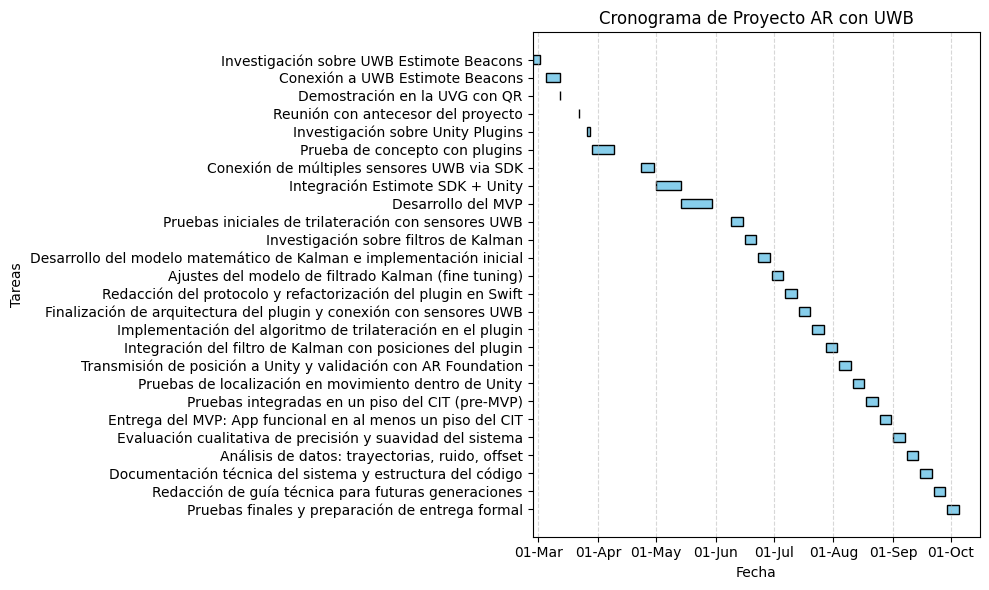
\includegraphics[width=1\textwidth]{images/cronograma3.png}
{\begin{center}
    Figura 1: Cronograma del proyecto.
\end{center}}
\newpage

    
 

\section{Bibliografía}
\begin{itemize} 
    \item Estimote, Inc. (n.d.). \textit{Estimote Location Beacons: UWB and BLE}. Estimote Documentation. Recuperado de: \url{https://developer.estimote.com/proximity/ultra-wideband/}
    
    \item Estimote, Inc. (n.d.). \textit{Estimote Proximity SDK}. Estimote Documentation. Recuperado de: \url{https://developer.estimote.com/proximity/ios-tutorial/}
    
    \item Unity Technologies. (n.d.). \textit{AR Foundation overview}. Unity Documentation. Recuperado de: \url{https://docs.unity3d.com/Packages/com.unity.xr.arfoundation@5.0/manual/index.html}
    
    \item Unity Technologies. (n.d.). \textit{Unity Manual: ARKit and ARCore with AR Foundation}. Recuperado de: \url{https://docs.unity3d.com/Manual/com.unity.xr.arfoundation.html}

    \item Apple Inc. (n.d.). \textit{Developing a Custom Unity Plugin for iOS}. Apple Developer / Unity Integration Guides. Recuperado de: \url{https://developer.apple.com/documentation/}
    
    \item Google. (n.d.). \textit{Bluetooth Low Energy overview}. Android Developers. Recuperado de: \url{https://developer.android.com/guide/topics/connectivity/bluetooth-le}
    
    \item Apple Inc. (n.d.). \textit{Core Bluetooth Overview}. Recuperado de: \url{https://developer.apple.com/documentation/corebluetooth}
    
    \item Hart, P. E., Nilsson, N. J., \& Raphael, B. (1968). \textit{A formal basis for the heuristic determination of minimum cost paths}. IEEE Transactions on Systems Science and Cybernetics, 4(2), 100–107. \url{https://doi.org/10.1109/TSSC.1968.300136}
    
    \item Thrun, S., Burgard, W., \& Fox, D. (2005). \textit{Probabilistic Robotics}. MIT Press.
    
    \item Welch, G., \& Bishop, G. (1995). \textit{An Introduction to the Kalman Filter}. University of North Carolina at Chapel Hill. \url{https://www.cs.unc.edu/~welch/media/pdf/kalman_intro.pdf}
    
    \item Ho, K. C., \& Xu, Y. T. (2004). \textit{An accurate algebraic solution for moving source location using TDOA and FDOA measurements}. IEEE Transactions on Signal Processing, 52(9), 2453-2463. \url{https://doi.org/10.1109/TSP.2004.832009}
    
    \item GitHub. (n.d.). \textit{Unity Plugin Development for iOS and Android}. Ejemplos de integración. Recuperado de: \url{https://github.com/Unity-Technologies/UnityNativePlugin}
\end{itemize}

\end{document}